\chapter{Introdução} % (fold)
\label{cha:introdu_o}

\section{Contextualização} % (fold)
\label{sec:contextualiza_o}

A Robótica é um campo de pesquisa multi-disciplinar, que envolve desde mecânica e eletrônica a algoritmos de inteligência artificial, visão computacional, aprendizado de máquina, teoria de grafos, dentre outras, oriunda de áreas como a engenharia mecânica, elétrica e ciência da computação.
Tem como foco o estudo e desenvolvimento de máquinas capazes de auxiliar seres humanos em diversos cenários.
Estas máquinas podem possuir um certo nível de inteligência, podendo tomar decisões de modo a completar as atividades que foram empregados.
% , podendo ser utilizadas em cenários onde humanos não poderiam estar, seja por alguma característica inóspita ou riscos de acidentes, por exemplo.

% Robôs são agentes automáticos, que podem ser implementados virtualmente, como um programa de computador, podendo possuir uma forma física, como um corpo mecânico.
% Estes são, atualmente, responsáveis pela execução de diversas tarefas que comumente eram realizadas manualmente, por humanos, mas que foram estudadas e abstraídas de modo que possam ser exercidas de forma autônoma.

No princípio, os robôs foram utilizados principalmente no âmbito industrial, no qual exerciam o ofício de manipulação e construção de itens em linhas de montagem (veículos, empacotamento), onde se encontravam fixos ao ambiente de trabalho, possuindo limitada área de atuação, com grande acurácia de operação (\cite{Rol2011}).
Porém, com o passar dos anos, os mesmos deixaram de ser somente manipuladores de base fixa e passaram a poder mover-se pelo ambiente, atingindo maiores áreas e ganhando outras aplicações.
Estes foram adotados em funções como as de vigilância e reconhecimento de regiões (\cite{Tanner2007, Sujit2013}), busca e resgate no caso de acidentes ou catástrofes (\cite{Casper2003, Murphy2004}), mapeamento (\cite{Tokekar2013}), detecção e rastreamento de alvos (\cite{Grocholsky2006}) e transporte de objetos (\cite{Michael2011, Fink2008}).

% Em relação ao uso residencial, apesar de ainda restrito, principalmente pelo valor associado aos mesmos, já existem diversos estudos com o uso de manipuladores móveis que tratam de tarefas domésticas, como controlar medicamentos, limpar a casa (\cite{Graf2004}), na assistência a idosos e paciente com dificuldade de locomoção (\cite{Harmo2005}).
% Na Figura \ref{fig:robos_casa_a} demonstrado um braço robótico que é capaz de realizar movimentos humanos manipulando um objeto (\cite{Kormushev2010}), outro exemplo é o robô Asimo (Figura \ref{fig:robos_casa_b}), que executa diversas tarefas, como abrir uma garrafa, correr, subir/descer escadas, identificar e se comunicar de forma quase humana, dentre outras.

% \begin{figure}[htpb]
% 	\centering
% 	\setlength{\fboxsep}{0pt}
% 	\begin{subfigure}[t]{0.45\textwidth}
% 		\centering
% 		\fbox{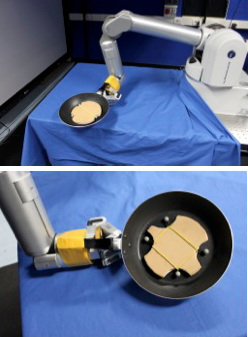
\includegraphics[height=0.28\textheight]{img/intro/hand.jpg}}
% 		\caption{}
% 		\label{fig:robos_casa_a}
% 	\end{subfigure}%
% 	\hspace{0.02cm}
% 	\begin{subfigure}[t]{0.45\textwidth}
% 		\centering
% 		\fbox{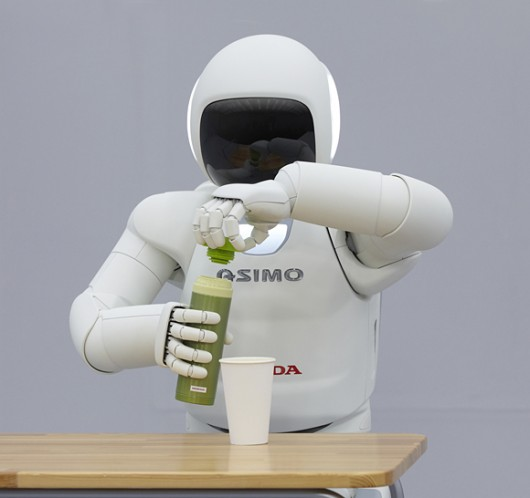
\includegraphics[height=0.28\textheight]{img/intro/asimo.jpg}}
% 		\caption{}
% 		\label{fig:robos_casa_b}
% 	\end{subfigure}
% 	\caption[Exemplos de Robôs manipuladores]{(a) Braço robótico capaz de realizar um movimento de 180º em um objeto (\cite{Kormushev2010}), (b) Robôs Asimo, capaz de executar diversas tarefas, como abrir uma garrafa (\cite{Sakagami2002}).}
% 	\label{fig:robos_casa}
% \end{figure}


Esta pluralidade de tarefas foi desenvolvida e melhorada com o uso de sistemas autônomos, agregando características como precisão, eficiência e eficácia em inúmeros aspectos (uso energético, diminuição do tempo de execução, custo financeiro, entre outros).

Uma das categorias nas quais o uso deste tipo de agente podem ser classificados diz respeito à quantidade de robôs empregados na tarefa, sendo estes de dois tipos: (i) sistemas de único robô (\de{srs} [\gl{srs}]) -- no qual um robô é responsável por toda a missão e deve possuir todos os recursos necessários para cumpri-la, e (ii) sistemas multi-robôs (\de{mrs} [\gl{mrs}]) -- onde um grupo de agentes, reunindo suas capacidades, exerce a função requerida em conjunto, de forma coordenada, aproveitando os recursos da equipe.

Comparativamente, um \gl{mrs}\ apresenta algumas vantagens em relação à utilização de um \gl{srs}, como uma maior robustez, menor taxa de falhas, além de diminuir em muitos casos o tempo necessário para realização da tarefa.
Uma vantagem notável do uso de times está na sua capacidade de realizar atividades complexas, como as descritas anteriormente, sem a necessidade de ser formado por agentes especializados para a tarefa, por exemplo, usando robôs mais simples para transportar um objeto ao invés de um único com um manipulador de alta tecnologia.

Outra particularidade somente encontrada em um \gl{mrs}, é que este pode atuar em ambientes nocivos ao ser humano, assim, poupando-o de qualquer acidente ou perigo que poderia ocorrer.
Exemplo este, é a utilização de grupos de busca e mapeamento aplicados em acidentes nucleares, como o ocorrido em Fukushima\footnote{\url{https://goo.gl/TJRYh9}}, utilizados para estudar o cenário após o desastre ocorrido, e fornecer informações à equipe humana a fim reduzir as consequências do mesmo.
Outros ambientes, como a inspeção de vulcões, locais com incêndio/fumaça, as profundezas do oceano são territórios indicados para adoção de robôs.

% Onde pode ser aplicado ?
Ao comparar o desempenho de algumas atividades sendo realizadas por agentes humanos e por agentes autônomos, é perceptível que a aplicação de um grupo de robôs pode agregar à tarefa qualidades (rapidez, acurácia, eficiência) que não poderiam ser alcançadas ou que seriam de grande custo para um time humano.

\section{Motivação} % (fold)
\label{sub:manipula_o_de_objetos}

O transporte e manipulação de objetos, apesar de transparecer ser uma tarefa simples, é de fundamental importância em diversas outras atividades, e requer o estudo de áreas como o planejamento de caminhos e a coordenação de agentes, quando é utilizado um \gl{mrs}, por exemplo.

Dentro do campo de pesquisa sobre manipulação usando robôs, além da classificação dos agentes entre os tipos fixos ou móveis (\cite{Rol2011}), os mesmos podem ser também agrupados considerando as estratégias usadas para mover e/ou portar o objeto, são elas: (i) não-preênsil (\emph{non-prehensile}) -- na qual o agente manipulador utiliza de ações como arremessar, rolar e/ou empurrar para completar o transporte do objeto, e (ii) preênsil (\emph{prehensile}) -- na qual o objeto a ser transportado é acolhido ou segurado pelo manipulador, que o leva até a posição final desejada e o deposita (\cite{Lynch1996,murray1994}).

A aplicabilidade de robôs capazes de manipular e transportar objetos tem crescido, principalmente buscando melhorar o rendimento e ganhos nas tarefa solicitadas.
Exemplos práticos deste uso podem ser vistos em cenários como: retirada de sedimentos em uma mina (\cite{Murphy2009}), realização de cirurgias (\cite{Lehman2008}), transporte de objetos (\cite{Michael2011}), manipulação de mercadorias em um armazém (\cite{Guizzo2008}), e na construção de bens e estruturas (\cite{Lindsey2012, BarrosdosSantos2013, BarrosdosSantos2014,Augugliaro2014}).

A Figura \ref{fig:transporte_robos} demonstra aplicações reais de transporte de objetos utilizando o modelo \gl{mrs}, considerando o uso de técnicas preênsil e não-preênsil.
Na Figura \ref{fig:transport_a} um grupo de agentes terrestres utiliza seu corpo para empurrar objetos por um ambiente (\cite{Fink2008}); a Figura \ref{fig:transport_b} demonstra o sistema de transporte de mercadoria \emph{Kiva} (\cite{Guizzo2008}), utilizado por grandes empresas como \emph{Amazon}\footnote{\url{http://www.amazon.com/}}, em seus armazéns. Utilizando um time de quadrotores, é possível construir estruturas baseado em segmentos pré-existentes (\cite{Lindsey2012}) ou com uso de blocos (\cite{Augugliaro2014}), visto na figuras \ref{fig:transport_c} e \ref{fig:transport_d}, respectivamente.

\begin{figure}[htpb]
	\centering
	\setlength{\fboxsep}{0pt}
	\begin{subfigure}[t]{0.49\textwidth}
		\centering
		\fbox{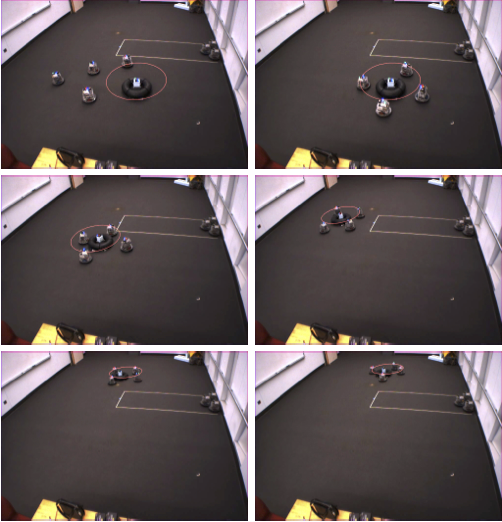
\includegraphics[height=0.29\textheight]{img/intro/ground_transport.png}}
		\caption{\cite{Fink2008}}
		\label{fig:transport_a}
	\end{subfigure}%
	\hspace{0.02cm}
	\begin{subfigure}[t]{0.49\textwidth}
		\centering
		\fbox{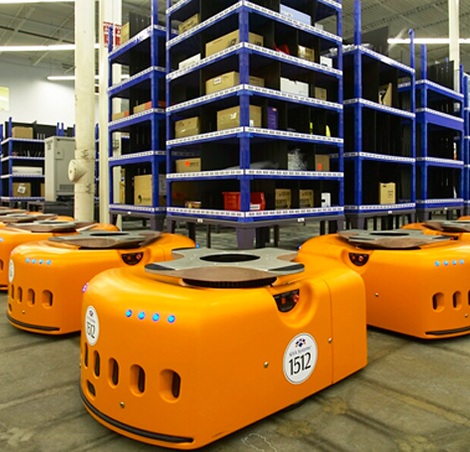
\includegraphics[height=0.29\textheight]{img/intro/kiva.png}}
		\caption{\cite{Guizzo2008}}
		\label{fig:transport_b}
	\end{subfigure}
	\vspace{0.3cm}

	\begin{subfigure}[t]{0.49\textwidth}
		\centering
		\fbox{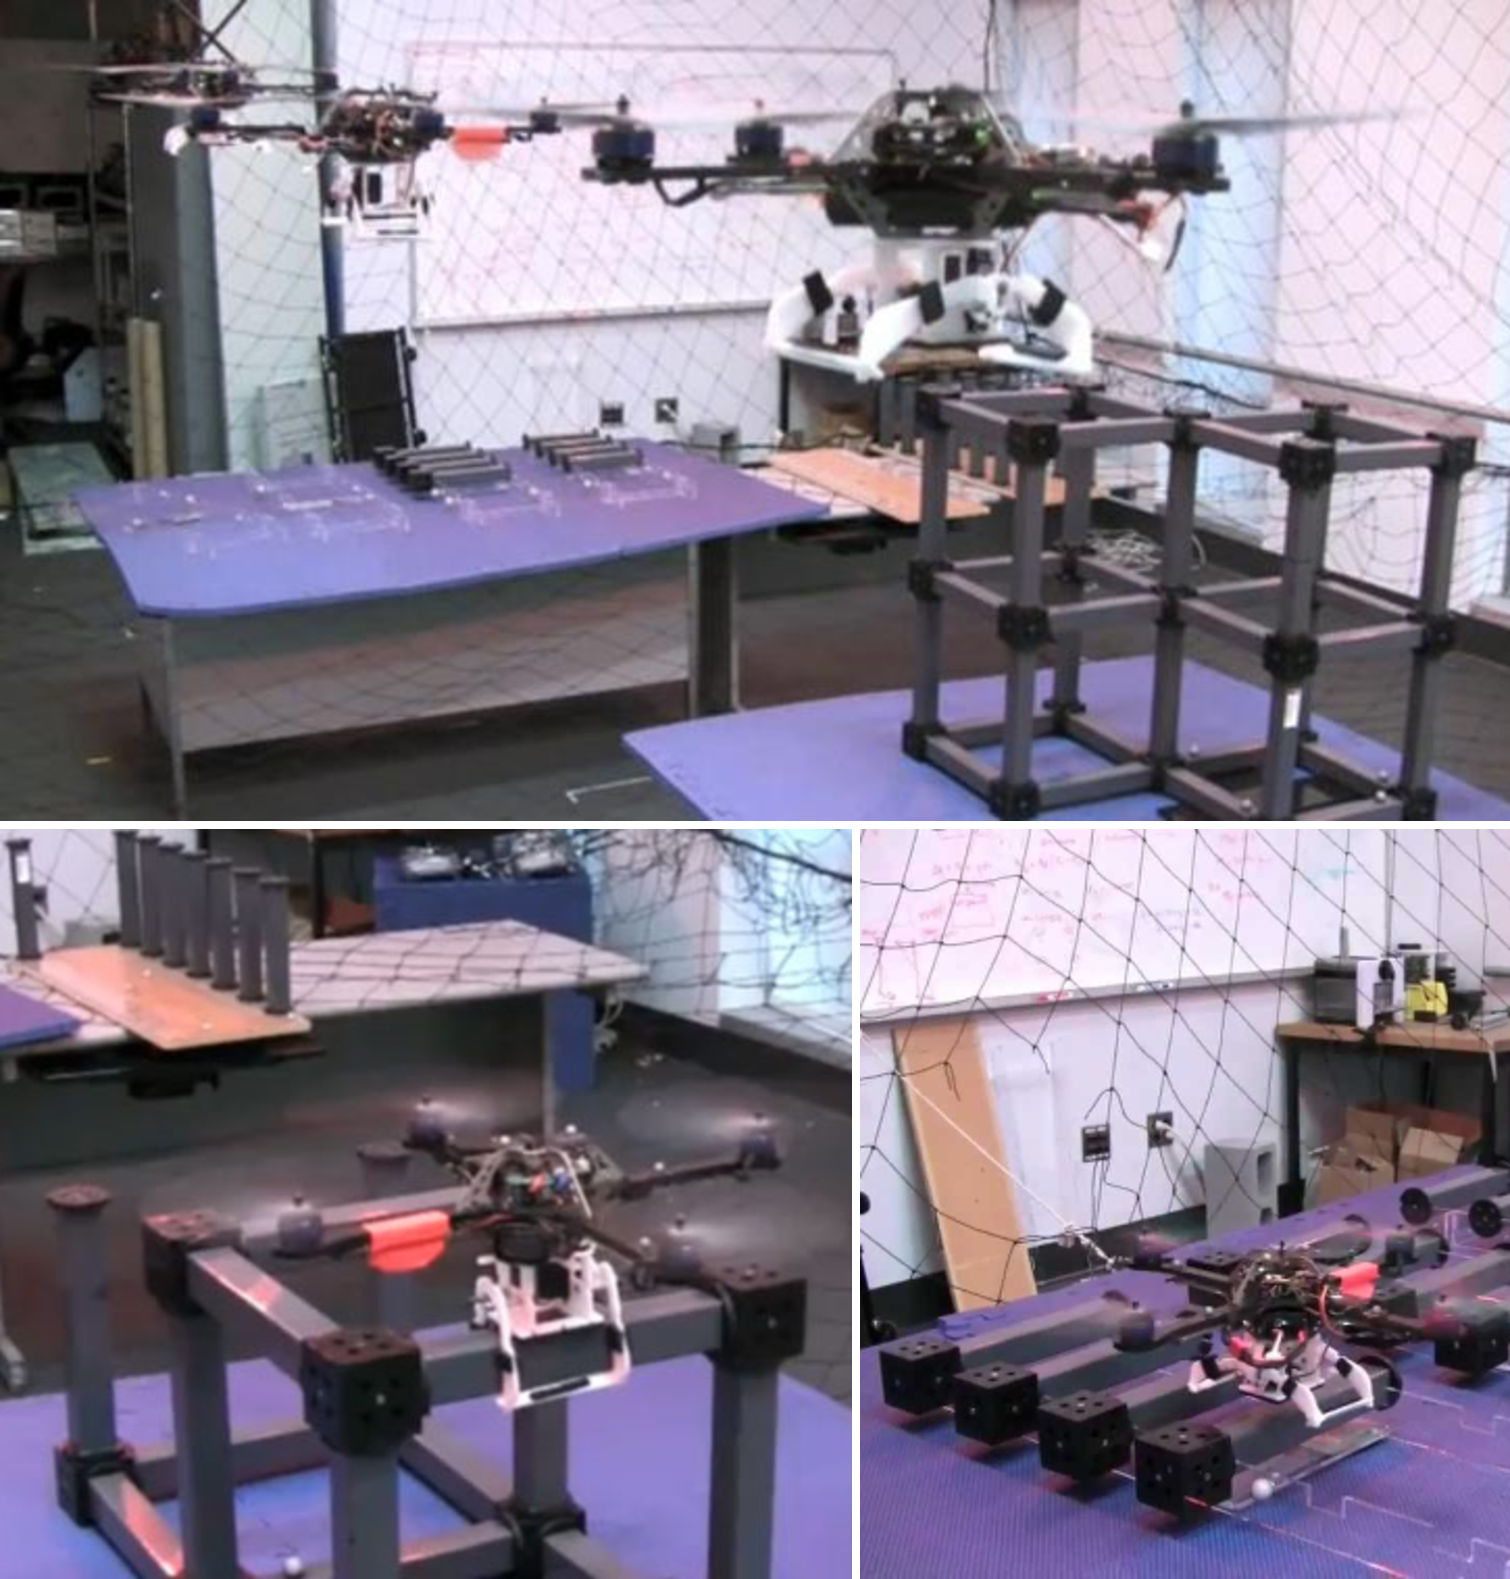
\includegraphics[height=0.29\textheight]{img/intro/quad_construction_3.pdf}}
		\caption{\cite{Lindsey2012}}
		\label{fig:transport_c}
	\end{subfigure}%
	\hspace{0.02cm}
	\begin{subfigure}[t]{0.49\textwidth}
		\centering
		\fbox{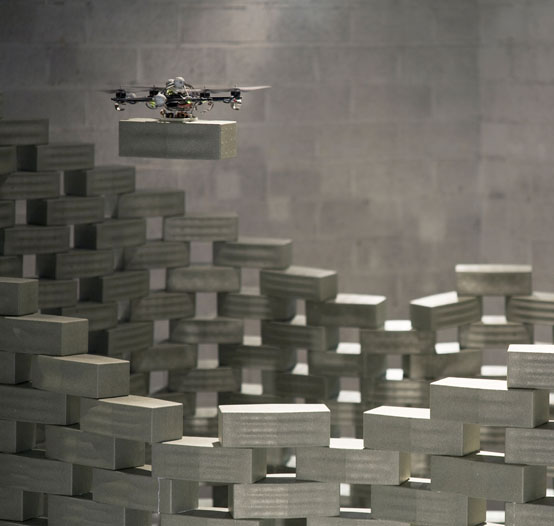
\includegraphics[height=0.29\textheight]{img/intro/quad_construction_2.jpg}}
		\caption{\cite{Augugliaro2014}}
		\label{fig:transport_d}
	\end{subfigure}
	\caption[Aplicações de Robôs para Transporte e Manipulação de Objetos]{Aplicações de sistemas robóticos desempenhando tarefas de transporte e manipulação de objetos. (a) -- um grupo de robôs utiliza seu corpo para mover objetos, (b) -- sistema de transporte \emph{Kiva}, (c) -- equipe de robôs usa segmentos para criar estruturas 3D, (d) exemplo de construção usando blocos e quadrotores.}
	\label{fig:transporte_robos}
\end{figure}

% \cite{Guizzo2008} KIVA
% \cite{Lindsey2012} construção
% \cite{Augugliaro2014} construção
% \cite{BarrosdosSantos2014,BarrosdosSantos2013} construção

% Por que fazer com um grupo de robôs ?
% Que ganhos ?

Em casos específicos, a realização da manipulação de objetos pode necessitar recursos que são indisponíveis ou que acarretariam em um aumento do custo total de execução se fosse realizado somente por um agente robótico, seja por que o mesmo não possui força mecânica suficiente ou pela tarefa necessitar de monitoramento externo durante, por exemplo.

% A aplicação de grupos de agentes (\mrs) para cumprir tal tarefa certamente é uma alternativa bastante plausível, pois garante ao arranjo diversas vantagens, apesar de aumentar a complexidade de controle.

Essencialmente, a utilização de uma equipe de agentes proporciona algumas vantagens, como: a diminuição no tempo necessário para realização de uma atividade, seja pela divisão das tarefas entre a equipe, seja pela execução de certas funções de forma conjunta; além de dispor de mais recursos (força física ou diversidade de capacidades), necessário para conclusão de algumas tarefas.
Baseado nestas propriedades, o uso de um time robótico tem se mostrado uma opção interessante em diversos contextos.

% Quais dificuldades do uso de um time ?

Apesar das evidentes qualidades de um \gl{mrs}, sua aplicação requer a adoção de técnicas mais complexas, principalmente no que se relaciona ao controle, coordenação e comunicação dos agentes, essencial para que a tarefa seja bem executada.

Questões fundamentais da robótica ainda se aplicam, porém em uma escala de maior complexidade.
Dentre esses problemas, destacam-se a localização, o planejamento de caminhos, a coordenação dos agentes e a própria forma em que a missão será realizada.

% O problema de localização está relacionado tanto ao agente em si quanto aos objetos no ambiente que se deseja transportar.
% O planejamento de caminhos pode ser abordado de diferentes maneiras, por exemplo com o objetivo de minimizar o tempo de transporte ou a energia gasta.
% Já a coordenação da equipe envolve questões de alocação de tarefas, bem como o estudo da combinação dos recursos disponíveis para realizar a atividade da melhor maneira possível.
%

% Neste sentido, são definidos os problemas que este trabalho apresenta propostas de soluções, no âmbito do uso de uma equipe heterogênea de agentes para o transporte de objetos dispostos em um ambiente.

\section{Problema} % (fold)
\label{sec:problema}

Este trabalho tem por objetivo apresentar uma metodologia para questões decorrentes do uso de uma equipe de agente robóticos, tendo como missão o transporte de objetos utilizando suas capacidades físicas e computacionais.
O problema específico tratado é descrito a seguir:

\begin{quotation}
Dado um grupo de agentes heterogêneos, executar a ação de transporte de um conjunto de objetos dispostos em um ambiente de trabalho discretizado, movendo-os de suas posições iniciais para suas respectivas posições finais previamente estipuladas, considerando os obstáculos presentes neste ambiente.
\end{quotation}

Para resolução do problema descrito, este trabalho apresenta uma proposta de solução mediante a criação de dois subproblemas, proporcionando uma melhor análise do mesmo, descritos a seguir:

\begin{description}

	\item[Problema 1] Planejamento de Caminhos do Objeto: Considerando o ambiente de trabalho no qual deve ocorrer o transporte, executar o planejamento de uma sequência de posições para cada objeto partindo de sua posição inicial com a finalidade de movê-lo até uma posição final desejada.
	Este plano deve evadir demais objetos e obstáculos no ambiente, bem como considerar as capacidades dos agentes disponíveis.
	Na Figura~\ref{fig:diagrama_problema_1} é demonstrado o resultado da solução deste problema, um caminho entre a pose inicial e a final.

	% Dado o ambiente de trabalho, estudar e descrever uma sequência de poses válidas para os objetos que garanta a chegada do mesmo à sua posição final desejada.

	\item[Problema 2] Alocação de Tarefas e Coordenação de Agentes: Considerando que o plano de manipulação dos objetos foi criado, este sub-problema se concentra na criação de um plano de execução dos agentes, contemplando a movimentação e as ações que os mesmos devem realizar para que o transporte seja completado.
	Uma vez que o plano de execução tenha sido criado, os agentes devem ser coordenados de forma que suas tarefas individuais estejam em sinergia, propiciando a realização da tarefa.
	A Figura~\ref{fig:diagrama_problema_2} demonstra um exemplo de coordenação para o transporte de um objeto, baseado no trajeto já determinado e dividindo as tarefas de acordo com os recursos de cada agente.

\end{description}

\begin{figure}[htpb]
	\centering
	\setlength{\fboxsep}{0pt}
	\begin{subfigure}[t]{0.32\textwidth}
		\centering
		\fbox{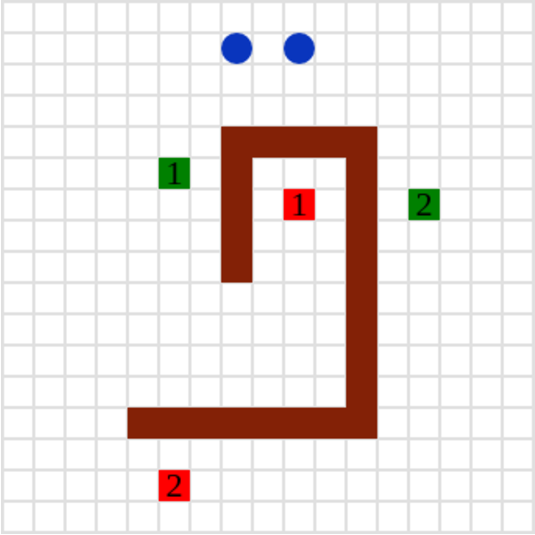
\includegraphics[width=\textwidth]{img/intro/intro_example_1.pdf}}
		\caption{Ambiente de trabalho para o transporte.}
		\label{fig:diagrama_problema_mapa}
	\end{subfigure}
	\hspace{0.02cm}
	\begin{subfigure}[t]{0.32\textwidth}
		\centering
		\fbox{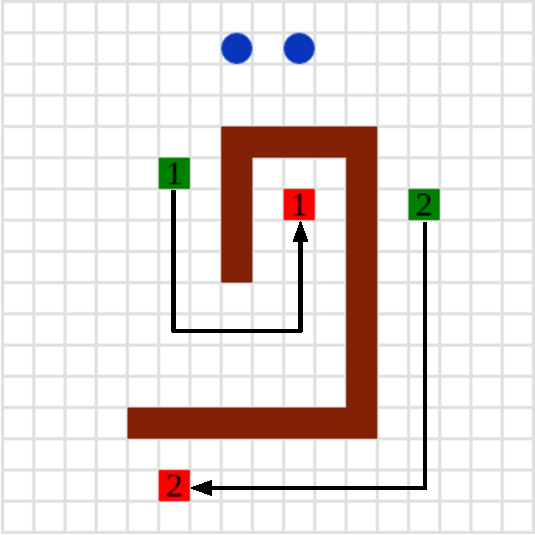
\includegraphics[width=\textwidth]{img/intro/intro_example_2.pdf}}
		\caption{Solução do Problema 1 - Planejamento para os objetos.}
		\label{fig:diagrama_problema_1}
	\end{subfigure}
	\hspace{0.02cm}
	\begin{subfigure}[t]{0.32\textwidth}
		\centering
		\fbox{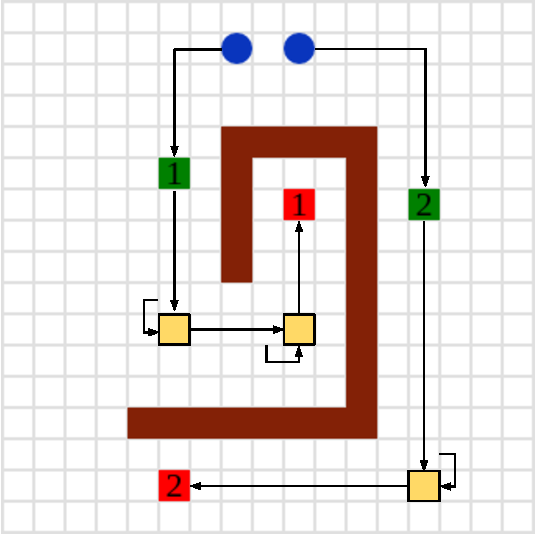
\includegraphics[width=\textwidth]{img/intro/intro_example_3.pdf}}
		\caption{Solução do Problema 2 - Planejamento e execução pelos agentes.}
		\label{fig:diagrama_problema_2}
	\end{subfigure}
	\caption[Uma solução do problema de transporte de objetos]{Solução do problema de transporte de objetos. Um mapa descrevendo o ambiente serve como ponto de entrada para o sistema (a), que na primeira etapa cria os planos de movimentação para os objetos (b), e posteriormente, os utiliza para criar planos para os agentes e coordená-los na execução (c).}
	\label{fig:diagrama_problema}
\end{figure}

% section problema (end)

\section{Contribuições} % (fold)
\label{sec:contribui_es}

Este trabalho apresenta técnicas para controle e coordenação de um conjunto de agentes robóticos incumbidos da realização das tarefas de manipulação e transporte de um conjunto de objetos.

O principal diferencial do trabalho apresentado é tratar o plano de movimentação do objeto a ser transportado como base para as demais etapas do processo, considerando que a maioria dos trabalhos que propõem soluções neste campo de pesquisa focam na movimentação dos agentes.

São apresentadas propostas nas diversas áreas envolvidas no processo de transporte: no planejamento de caminhos, no qual uma função de utilidade, que pondera dimensões como tempo de travessia e energia, é utilizada para encontrar o melhor plano, além de demonstrar estudos sobre a penalização das mudanças de direção dos objetos; a etapa de alocação de tarefas entre os agentes é realizada de forma descentralizada e coordenada; e finalmente, para a execução da missão é demonstrado um algoritmo baseado em estratégias de redes de computadores, para sincronizar e sistematizar os agentes durante a resolução da tarefa.

Parte desta metodologia, que se concentra no planejamento e transporte dos objetos juntamente com a técnica de penalização utilizando um agente, foi publicada na Conferência LARS 2015 -- \emph{12th Latin American Robotics Symposium} e SBR 2015 -- 3º Simpósio Brasileiro de Robótica, sob o título \emph{Multi-object Transportation using a Mobile Robot} (\cite{Melo2015}), demonstrando que este tema é relevante para a comunidade pesquisadora de robótica.

\section{Organização do Trabalho} % (fold)
\label{sec:organiza_o_do_trabalho}

O presente trabalho está organizado da seguinte forma, o Capítulo \ref{cha:trabalhos_relacionados} apresenta o estado da arte nas diversas áreas que compreendem o mapeamento, planejamento e coordenação de robôs.
No Capítulo \ref{cha:metodologia} é apresentada a metodologia utilizada durante a criação e experimentação das soluções trabalhadas, seguido dos experimentos e validações realizadas no Capítulo \ref{cha:experimentos}.
Por fim, concluímos no Capítulo \ref{cha:conclus_o} este trabalho com assertivas acerca da capacidade de aplicação da técnica apresentada bem como de sua importância perante outros trabalhos.

% section organiza_o_do_trabalho (end)

% chapter introdu_o (end)
